% credit goes to stamford university project template
\documentclass[11pt]{report}
\usepackage{mathptmx}
\renewcommand{\familydefault}{\rmdefault}
\usepackage[a4paper]{geometry}
\geometry{verbose,tmargin=2cm,bmargin=2cm,lmargin=2cm,rmargin=2cm,headheight=1cm,headsep=1cm,footskip=1cm}
\setcounter{secnumdepth}{3}
\setcounter{tocdepth}{3}
\setlength{\parskip}{\medskipamount}
\setlength{\parindent}{0pt}
\usepackage[numbers]{natbib}
\usepackage{verbatim}
\usepackage{pdfpages}
\usepackage{graphicx}
\usepackage{setspace}
\usepackage[numbers]{natbib}
\usepackage{nomencl}
\usepackage{multirow}
\usepackage{listings}
\usepackage[breakable,skins]{tcolorbox}
\usepackage{float}
\usepackage[titles]{tocloft}
%%  Changing indentation  of chapter title in toc
\makeatletter
\renewcommand{\numberline}[1]{%
  \setbox0\hbox{#1\quad}%
  \hb@xt@\wd0{\@cftbsnum #1\@cftasnum\hfil}\@cftasnumb}
\makeatother

% the following is useful when we have the old nomencl.sty package
\providecommand{\printnomenclature}{\printglossary}
\providecommand{\makenomenclature}{\makeglossary}
\makenomenclature
\doublespacing

\makeatletter

%%%%%%%%%%%%%%%%%%%%%%%%%%%%%% LyX specific LaTeX commands.
\providecommand{\LyX}{L\kern-.1667em\lower.25em\hbox{Y}\kern-.125emX\@}
%% Because html converters don't know tabularnewline
\providecommand{\tabularnewline}{\\}
%% A simple dot to overcome graphicx limitations
\newcommand{\lyxdot}{.}


%%%%%%%%%%%%%%%%%%%%%%%%%%%%%% User specified LaTeX commands.
\usepackage{tauthesis}
\usepackage[font={small,bf}, labelfont={small,bf}, margin=1cm]{caption}
\usepackage{titlesec}
\newcommand{\hsp}{\hspace{20pt}}

\titleformat{\chapter}[hang]{\Huge\bfseries}{\thechapter\hsp}{0pt}{\Huge\bfseries}
\Degreetext{\emph{A Project Report Submitted in Partial Fulfillment of the Requirements for the Degree of}}
\Title{\textbf{Heart Diagnosis Requirement Predictor}}
\Author{\textbf{Sujoy Das} \\gau-c-17/054 \\ \ \\ \textbf{Prastuti Koch} \\ gau-c-17/289 \\ \ \\ \textbf{Shivam Gupta} \\ gau-c-17/071
\\ \vspace{1cm}
Supervised by: \\Sanjib Narzary \\Assistant Professor
}
\Year{September 2020}
\Supervisor{Sanjib Narzary}
\Department{Department of Computer Science \& Engineering}
\Degree{Bachelors Degree in Computer Science \& Engineering}
%\Degree{Bachelor of Technology \\in\\ Computer Science \& Engineering}
% \Degree{Bacehlor of Technology}

\makeatother

\usepackage[english]{babel}
\begin{document}

\prelimpages

\titlepage



\chapter*{Abstract}
Abstract text here....


\approval{
The Project Report ``Heart Diagnosis Requirement Predictor'' submitted by Sujoy Das: gau-c-17/054, Prastuti Koch: gau-c-17/289 and Shivam Gupta: gau-c-17/071 to the Department of Computer Science \& Engineering, Central Institute of Technology, Kokrajhar, has been accepted as satisfactory for the partial fulfillment of the requirements for the degree of Bachelor of Technology in Computer Science \& Engineering and approved as to its style and contents. \\

\vspace*{20pt}
\noindent Board of Examiner's Name, Signature, and Date:\\\\

\noindent \minipage{0.32\textwidth}
  ........................................... \\ \\
\textbf{(Board Member 1) } \\ 
Date: \\

\endminipage\hfill
\minipage{0.32\textwidth}
........................................... \\ \\
\textbf{(Board Member 2) } \\ 
Date: \\
\endminipage\hfill
\minipage{0.32\textwidth}%
........................................... \\ \\
\textbf{(Board Member 3) } \\ 
Date: \\
\endminipage

\vspace*{20pt}
\noindent Supervisor's Signature and Date:\\\\
........................................... \\
\textbf{Sanjib Narzary} \\ \\
Date: 


}

\declaration{
We, hereby, declare that the work presented in this Thesis / Project is the outcome of the investigation performed by us under the supervision of Sanjib Narzary, Assistant Professor, Department of Computer Science \& Engineering, Central Institute of Technology, Kokrajhar. We also declare that no part of this Project and thereof has been or is being submitted elsewhere for the award of any degree or Diploma. \\

\vspace*{20pt}
\noindent Signature and Date: \\\\
........................................... \\
\textbf{Sujoy Das} \\
Date: \\\\
........................................... \\
\textbf{Prastuti Koch} \\
Date: \\\\
........................................... \\
\textbf{Shivam Gupta} \\
Date: \\

}

\dedication{
Dedicated to ...
}

\acknowledgments{
Acknowledgement text here...
}


%\tableofcontents{}
\tableofcontents

\textpages

\listoffigures

\listoftables

\printnomenclature{}

%\footnote{Split the thesis into separate chapters. Use \textbackslash{}include mode to include the separate files.}


\chapter{Introduction}
Introduction text here...

\section{Motivation}
Motivation text here... 

\section{Sensors}
\begin{enumerate}
\item ESP8266 12E wi-fi/Node MCU	
\item 4/8/16 channel Relay Board				
\item USB TTL Serial Adapter
\item PIR Motion sensors 
\end{enumerate}

\subsection{Thermostats and HVAC controls}
Common thermostats and HVAC controls  are:
\begin{itemize}
\item 	Humidity sensing and control  
\item 	Temperature sensors and controllers    
\item 	Weather stations and sensors  
\end{itemize}

\subsection{Example Figure}
An example figure insertion is presented  in  Figure \ref{fig1}.

\begin{figure}[H]
\begin{center}
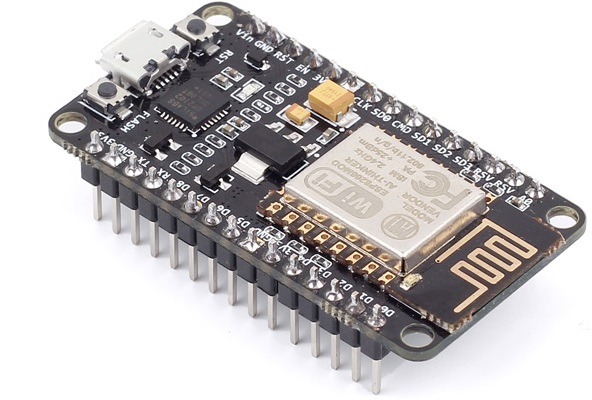
\includegraphics[width=0.8\textwidth]{fig1}
\end{center}
\caption{NodeMCU Microcontroller}
\label{fig1}
\end{figure}

\subsection{Example Referencing}
An example of inserting references in latex \cite{7890229} \cite{swapnil2016}. 

\section{Chapter Summary}
In this chapter, .....  

\chapter{Literature Review}
Chapter introductory text here ...   

\section{Background Study}
Refer all background study like here \cite{elshafee2012design}. Few more references inserted here \cite{harper2006inside} \cite{7887698}. Web sites can  also be put as reference like here \cite{arduino-ide}. 

\subsection{Android-based Home Automation}
An example of Android-based home automation system \cite{Agarwal} is presented in  Figure \ref{fig2}.  
\begin{figure}[htp]
\begin{center}
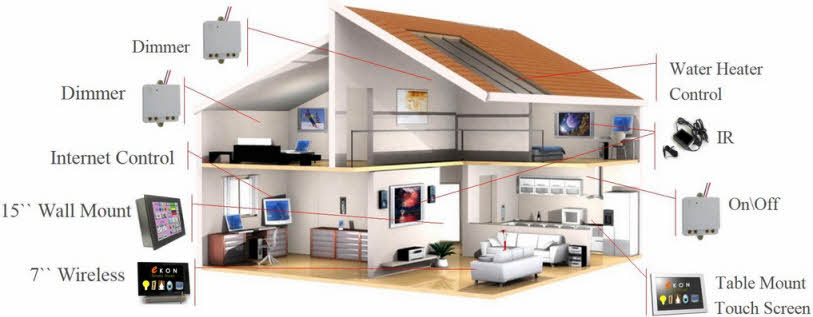
\includegraphics[width=0.8\textwidth]{fig2}
\end{center}
\caption{Android-based home automation system}
\label{fig2}
\end{figure}


\section{Chapter Summary}
In this chapter,  ....


\chapter{System Design}
Chapter introductory text here ...

\subsection{Pin Definition}
In the Figure \ref{fig-pin}, the pin definition of NodeMCU \cite{nodemcu2014} is shown and in  the Table \ref{table1} a detailed pin description is given. 
 
\begin{figure}[H]
\begin{center}
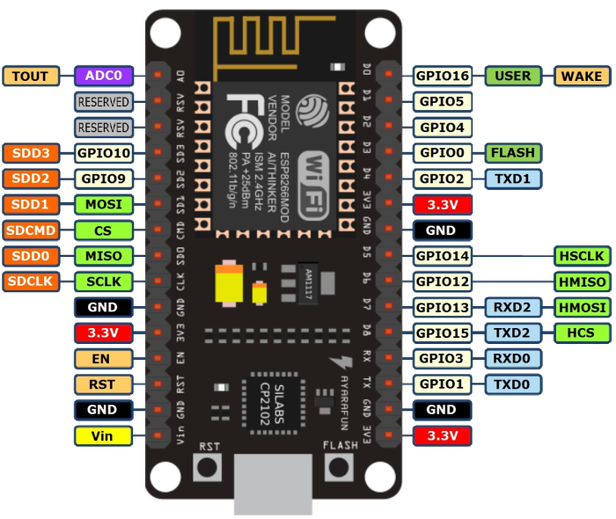
\includegraphics[width=0.66\textwidth]{figpin}
\end{center}
\caption{Pin Definition of NodeMCU}
\label{fig-pin}
\end{figure}

\begin{table}
\centering
\caption{Pin Description of NodeMCU}
\label{table1}
\begin{tabular}{|l|l|l|p{8cm}|}
\hline 
\textbf{Pin} & \textbf{Name} & \textbf{Type} & \textbf{Function} \tabularnewline
\hline 
1 & VDDA & P & Analog Power 3.02 \~ 3.6 V \tabularnewline \hline 
2 & LNA & I/O & RF Antenna Interface. Chip Output Impedance=50$\Omega$ No matching required but we recommend that the $\pi$-type matching network is retained. \tabularnewline \hline 
3 & VDD3P3 & P & Analog Power 3.02 \~ 3.6 V \tabularnewline \hline 
4 & VDD3P3 & P & Analog Power 3.02 \~ 3.6 V \tabularnewline \hline 
5 & VDD3P3 & P & Analog Power 3.02 \~ 3.6 V \tabularnewline \hline 
6 & ... & ... & ... \tabularnewline \hline 
\end{tabular}
\end{table}


\section{Parameter}
The NodeMCU parameters are listed in Table \ref{table2}.

\begin{table}
\caption{Parameters of NodeMCU}
\label{table2}
\centering
\begin{tabular}{|l|p{3.7cm}|p{4.8cm}|}
\hline 
\textbf{Categories} & \textbf{Items} & \textbf{Values} \tabularnewline
\hline 
\multirow{1}{*}{Wi-Fi Parameters} & certificates & FCC/CE/TELEC/SRRC \\\cline{2-3}
                 & WiFi Protocols & 802.11 b/g/n \\\cline{2-3}
                 & Frequency Range	 & 2.4G-2.5G (2400M-2483.5M) \\\cline{2-3}
                 & \multirow{2}{*}{TX Power} & 802.11 b: +20 dBm \\\cline{3-3}
                 & & 802.11 g: +17 dBm \\ \cline{3-3}
                 & & 802.11 n: +14 dBm \\ \cline{2-3}
                 & \multirow{2}{*}{RX Sensitivity} & 802.11 b: -91 dbm (11 Mbps)   \\\cline{3-3}
                 & & 802.11 g: -75 dbm (54 Mbps)  \\ \cline{3-3}
                 & & 802.11 n: -72 dbm (MCS7) \\ \cline{2-3}
                   & Types of Antenna & PCB Trace, External, IPEX Connector, Ceramic Chip    \\ \cline{1-3}
                 
\multirow{1}{*}{Hardware Parameters} & \multirow{2}{*}{TX Power} & UART/SDIO/SPI/I2C/ \newline I2S/IR Remote Control \\\cline{3-3}
                 &  & GPIO/PWM\\\cline{2-3}                
                 & Operating Voltage & 3.0~3.6V \\ \cline{2-3}
                 & Operating Current & Average value: 80mA \\ \cline{2-3}
                 & Operating Temperature Range& -40°~125° \\ \cline{2-3}
                 & Ambient Temperature Range & Normal temperature  \\\cline{2-3}
                 & Package Size & 5x5mm  \\ \cline{2-3}
                 & External Interface & N/A \\ \cline{1-3} \hline 
\end{tabular}
\end{table}

\section{Chapter Summary}
In this chapter, ...














\chapter{Implementation}
Chapter introductory text here ...

\section{Implementation}
...

\subsection{Configuration Code}
Sample configuration code  is  presented  in  
\lstset{language=c, showstringspaces=false, tabsize=1, breaklines=true, breakatwhitespace=false, framexleftmargin=20pt,numbers=left, 
numberstyle=\small,numbersep=10pt,frame=single,captionpos=t,xleftmargin=.061\textwidth}
\begin{center}
\begin{lstlisting}[caption=NodeMCU Configuration Code, label=nodemcuconfig]
#define BLYNK_PRINT Serial   
#include <ESP8266WiFi.h>
#include <BlynkSimpleEsp8266.h>

char auth[] = "YourAuthToken";

char ssid[] = "YourNetworkName";
char pass[] = "YourPassword";
void setup()
{
Serial.begin(115200);
Blynk.begin(auth, ssid, pass);
}
void loop()
{ Blynk.run(); }

\end{lstlisting}
\end{center}


\section{Chapter Summary}
In this chapter, ...






\chapter{Conclusion}
Conclusion text here ...

\section{Limitations}
...
\section{Future Works}
...











%if not needed use % to comment
%include{chapters/doesnotexit}


%\bibliographystyle{plainnat}
%\bibliographystyle{IEEEtran}
\bibliographystyle{IEEEtranN}
\bibliography{references}


\appendix
%
\chapter{Appendix title}

Appendix is just a different type of Section - it's included at the
end of the document (after the bibliography or list of references)
and before the Hebrew part and it's numbered in a different manner. 


\newpage{}

\end{document}